% PrepAIred IEEE conference paper -- anonymous/double-blind source.
%
% NOTE ON VERIFICATION STATUS (read before use): this .tex file is a
% content-equivalent, secondary artifact. No LaTeX distribution (pdflatex /
% xelatex / latexmk) was available in the build environment used for this
% deliverable, so this file has NOT been locally compiled and its resulting
% page count has NOT been verified here. The authoritative, page-verified
% deliverable is Final_IEEE_Paper_Anonymous.pdf, built from the official IEEE
% Word conference template and directly measured at 5 pages (see
% IEEE_Page_Limit_Verification.md). Before relying on this .tex file, compile
% it with the standard IEEEtran class (conference mode) and re-verify the
% page count and layout yourself -- do not assume parity with the Word build
% without checking, since font metrics and line-breaking differ between the
% two toolchains.
\documentclass[conference]{IEEEtran}
\IEEEoverridecommandlockouts
\usepackage{cite}
\usepackage{amsmath,amssymb,amsfonts}
\usepackage{graphicx}
\usepackage{booktabs}
\usepackage{url}

\begin{document}

\title{PrepAIred: Architecture and Evidence-Based Evaluation of a Guardrail-Shielded Adaptive Technical-Interview System}

\author{
\IEEEauthorblockN{Anonymous Author(s)}
\IEEEauthorblockA{Anonymous Affiliation \\ Submitted for double-blind review}
}

\maketitle

\begin{abstract}
Technical-interview preparation tools typically present fixed-difficulty question pools and coarse, unexplained scoring, providing no individualized adaptation or actionable feedback. We present PrepAIred, a deployed system that pairs a rubric-anchored, three-component answer evaluator (semantic similarity, concept-coverage retrieval, and a fine-tuned cross-encoder reasoning score) with a Proximal Policy Optimization (PPO) difficulty controller shielded by a deterministic, priority-ordered guardrail layer, and a locally hosted language model confined to narrative feedback generation. We report four independently verified findings from this system's evidence record. First, the evaluator's composite score correlates with human judgment at Spearman $\rho = 0.3812$ (95\% CI [0.158, 0.577]; 3 raters, 64 answers), a moderate, exploratory result reported with its full uncertainty rather than a stronger historical figure. Second, direct code-path tracing confirms the language model never computes or adjusts the numeric score, addressing a standard objection to LLM-involved evaluators. Third, a matched, multi-seed baseline comparison and a pre-registered confirmatory test find that the trained PPO policy's contribution to difficulty-tracking accuracy, over a trivial constant action under the same guardrail shield, is not statistically distinguishable from zero -- the guardrail layer, not the learned policy, accounts for the system's measurable adaptive behavior. Fourth, systematic boundary testing of the deployed guardrail layer surfaced and enabled correction of a genuine safety-coverage gap. We report all four findings, favorable and unfavorable, with identical evidentiary rigor.
\end{abstract}

\begin{IEEEkeywords}
adaptive interview preparation, reinforcement learning, large language models, automated answer evaluation, semantic similarity, equivalence testing, software guardrails
\end{IEEEkeywords}

\section{Introduction}

Existing technical-interview preparation tools present a fixed sequence of questions at fixed or self-selected difficulty, score answers through binary or coarse numeric checks where scoring exists at all, and provide no structured explanation of why an answer was scored as it was \cite{weiss1982}. This leaves two populations poorly served: candidates whose demonstrated skill exceeds the question pool's difficulty, and candidates for whom the pool offers no scaffolded path to improvement. Difficulty adaptation has a long history in testing theory \cite{weiss1982} and intelligent tutoring \cite{anderson1995,corbett1994}, but applying a \emph{learned} policy to this decision -- rather than a fixed item-response model -- raises a question that is rarely examined once such a system is deployed: once a learned policy is paired with a deterministic safety layer meant to catch its unsafe recommendations, does the learned component actually add measurable value over the safety layer alone?

We present PrepAIred, a deployed adaptive technical-interview system for C-language and data-structures practice. The system combines a rubric-anchored, three-component answer evaluator; a frozen Proximal Policy Optimization (PPO) \cite{schulman2017} policy that proposes difficulty adjustments; a six-rule deterministic guardrail layer that may override that proposal; and a locally hosted language model used only for narrative feedback. Unlike prior adaptive-interview and automated-scoring work, which typically reports only aggregate accuracy or user-study outcomes, we report this system's full evidence record -- including an unfavorable result for the learned policy -- because the methodological apparatus needed to detect that result honestly (multi-seed training, matched baselines, a pre-registered confirmatory test) is itself a reusable contribution for any system that pairs a learned component with a deterministic safety shield.

\textbf{Contributions.} (1) A deployed, single-controller system architecture combining a three-component composite evaluator, a guardrail-shielded RL difficulty controller, and a scope-limited feedback LLM, with every component's role independently verified against the implementation rather than assumed from its design intent. (2) An exploratory but methodologically disclosed human-correlation validation of the composite evaluator ($\rho = 0.3812$, 3 raters, 64 constructed answers), including a component ablation and a trivial-baseline comparison that contextualizes the result honestly. (3) A matched, multi-seed baseline comparison and pre-registered confirmatory equivalence test isolating the learned policy's marginal contribution from the guardrail layer's -- finding no detectable contribution from the policy alone, and reporting this as a legitimate equivalence result rather than omitting it. (4) A direct, code-level verification that the system's embedded language model never influences the numeric score, and a boundary-testing methodology that found and closed a genuine safety-coverage gap in the deployed guardrail layer.

\textbf{What we do not claim.} We make no claim of real-candidate learning-outcome improvement (all RL training and evaluation is simulation-based); we do not claim the evaluator is validated at publication-grade confidence (the human-correlation study is small and exploratory, stated as such throughout); and we do not claim architectural novelty in any single component -- our contribution is the system's integration and, centrally, the rigor and honesty of its own evaluation.

\section{Related Work}

\textbf{Automated and LLM-assisted scoring.} AutoSCORE \cite{wang2025} decomposes essay scoring across specialist agents coordinated by a rubric-aligned validating agent, outperforming monolithic LLM scoring; independent studies \cite{karjus2026,mendonca2025} find LLM-based scoring reliable but prompt- and domain-dependent. PrepAIred's evaluator follows a structurally related pattern -- three deterministic, fixed-weight scoring components rather than an LLM judge -- motivated by the same reliability concern: a generative component is used only as a secondary, scope-limited signal (feedback text), never as the primary scorer, which we verify directly rather than assert (\S\ref{sec:qwen}, \S\ref{sec:qwenverif}).

\textbf{Grounded verification.} Argos \cite{argos2026} shows that grounding a reward or verification signal in independently checkable evidence, rather than a learned component's own output, reduces hallucination-driven error in agentic reinforcement learning. The same principle motivates PrepAIred's design (a deterministic evaluator as the scoring path of record) and this paper's own verification discipline.

\textbf{Multi-agent coordination evaluation.} MultiAgentBench \cite{zhu2025} establishes milestone-based evaluation for multi-agent coordination quality rather than end-to-end completion alone. PrepAIred is a single-controller system with no inter-agent arbitration; we cite this work only for its evaluation-methodology principle, applied here at the guardrail/policy boundary.

\textbf{Curriculum and difficulty adaptation.} Automated curriculum learning \cite{graves2017,portelas2020} and intelligent-tutoring knowledge tracing \cite{anderson1995,corbett1994} both motivate using a learned policy to sequence task difficulty. PrepAIred's RL controller follows this tradition; our contribution is a rigorous test of whether that algorithm, once deployed behind a safety shield, performs the identified adaptive work.

\textbf{Multimodal interview analysis.} Prior work analyzes interview performance from video and multimodal features \cite{naim2015,chen2017}. PrepAIred captures audio-derived confidence and hesitation signals but, by design, no video or facial analysis -- a deliberate, disclosed scope limitation.

\textbf{Gap addressed.} No work we are aware of reports a pre-registered, confirmatory equivalence test isolating a deployed learned policy's marginal contribution from a deterministic safety layer wrapped around it, nor pairs that test with an equally rigorous, equally honestly reported evaluator-validation study for the same deployed system. This paper reports both.

\section{System Architecture}

PrepAIred is a single-controller, hub-and-spoke architecture (Fig.~\ref{fig:arch}). A central orchestrator owns all session state and mediates every other component. A React frontend communicates over a persistent connection for live interview turns. The composite evaluator scores verbal and code answers (\S\ref{sec:eval}). The speech pipeline produces a transcript plus prosodic confidence and hesitation signals. The strategy component proposes a difficulty action via the frozen PPO policy, which the guardrail layer may override (\S\ref{sec:rl}); the resulting action selects the next question via deterministic nearest-difficulty matching -- not semantic retrieval, a distinction verified directly against the implementation. A locally hosted language model generates narrative feedback, hints, and follow-up questions only after scoring completes (\S\ref{sec:qwen}). Code submissions execute in an isolated, resource-limited container that fails closed if the container runtime is unavailable. All session and turn data persist to a relational store with verified referential integrity.

\begin{figure}[t]
\centering
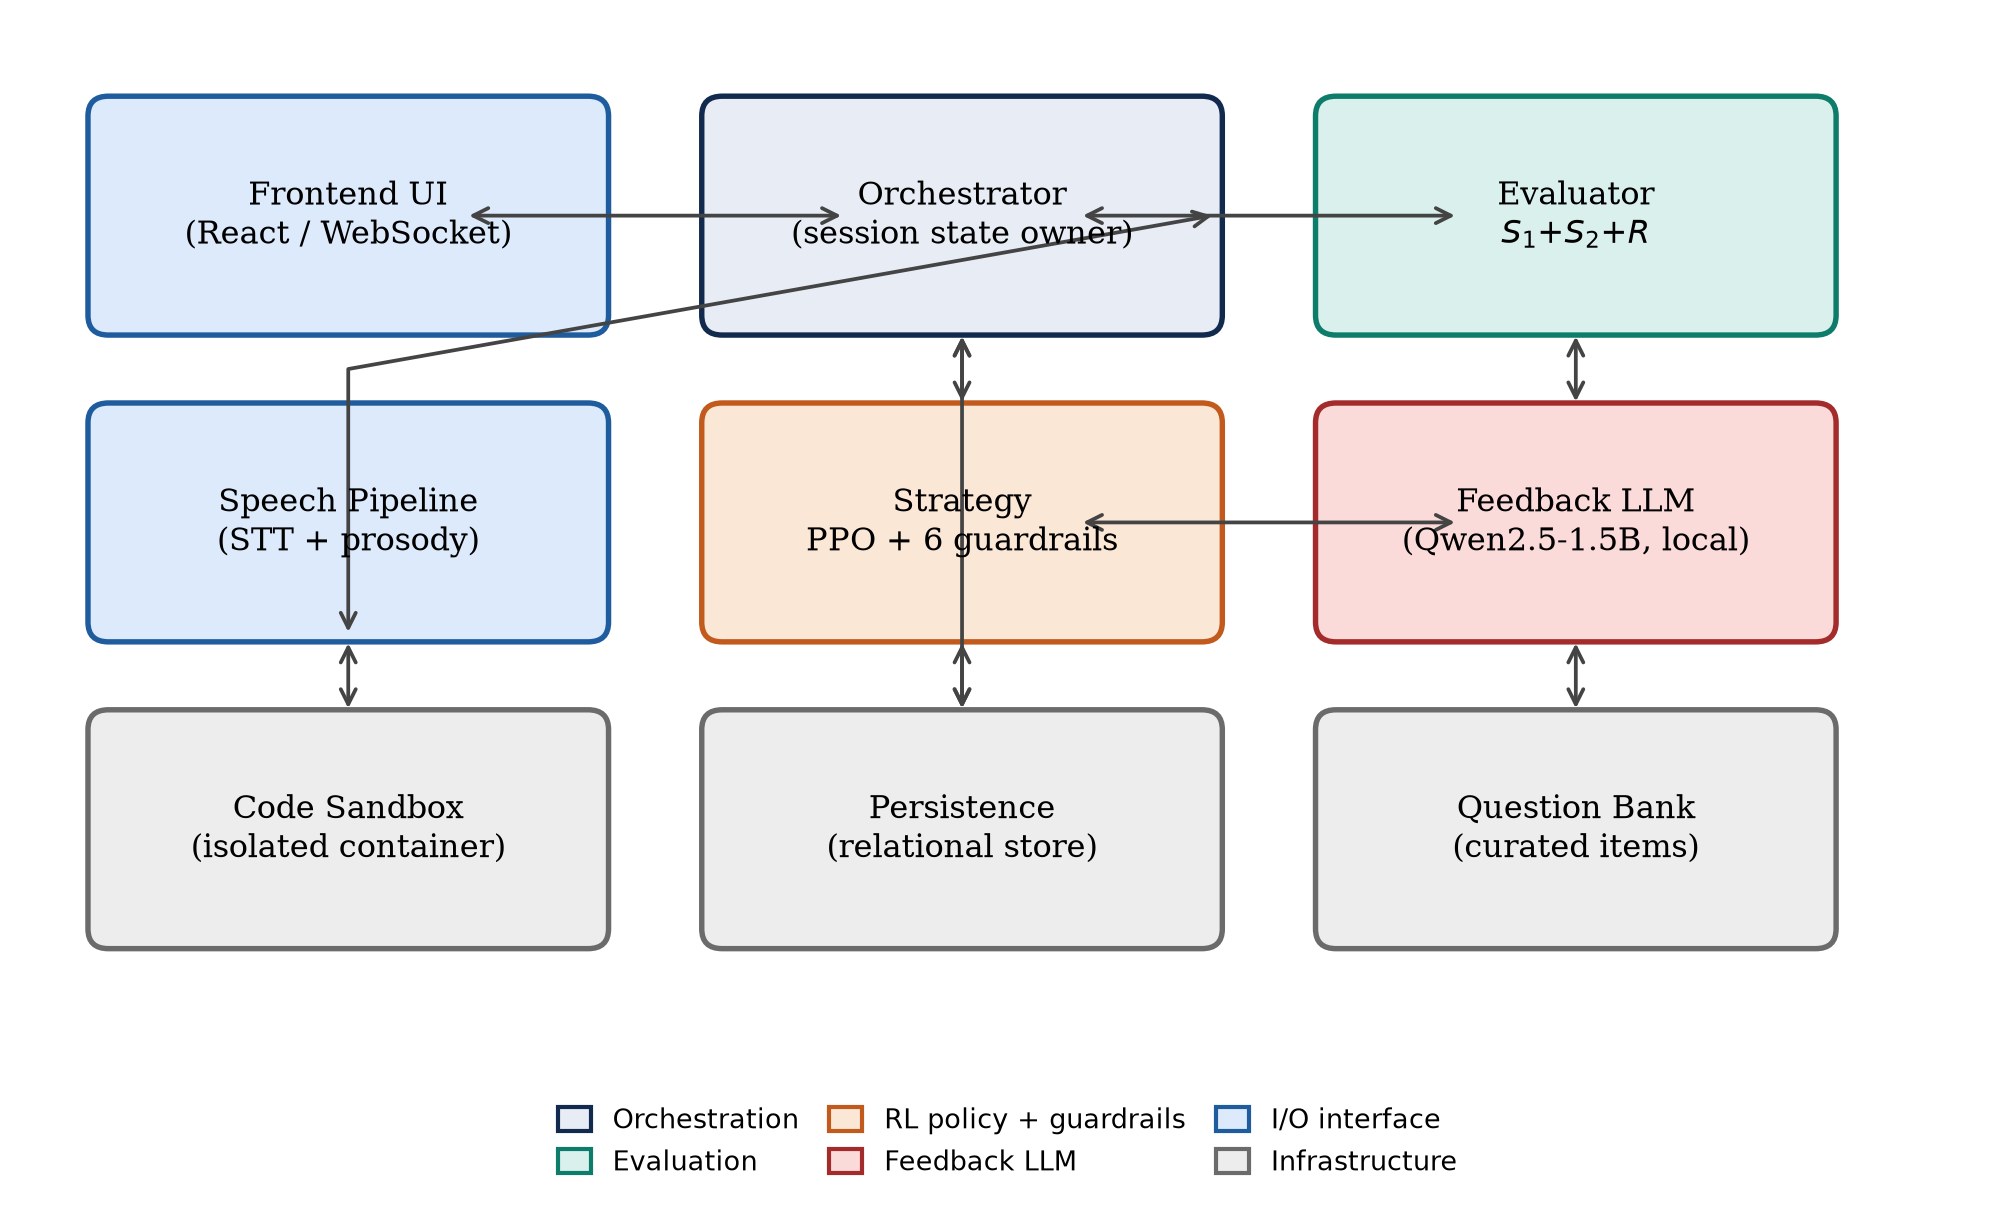
\includegraphics[width=0.85\linewidth]{IEEE_Figures/fig1_architecture.png}
\caption{PrepAIred system architecture. Arrows indicate verified data/control flow between the nine major components; there is no inter-agent arbitration layer.}
\label{fig:arch}
\end{figure}

\section{Methodology and Formulation}

\subsection{Composite Answer Evaluation}
\label{sec:eval}

Given a candidate answer split into sentences $\mathrm{Sent}(a)$ and a rubric for the current question, the evaluator computes three component scores. The semantic score averages, over each rubric semantic target $c$, the best cosine similarity to any candidate sentence embedding:
\begin{equation}
S_1 = \mathrm{mean}_{c \in C} \left[ \max_{s \in \mathrm{Sent}(a)} \cos(e(s), e(c)) \right]
\end{equation}
where $e(\cdot)$ is a Sentence-BERT embedding \cite{reimers2019}. The concept-coverage score is the fraction of rubric concepts whose best-matching sentence similarity exceeds a fixed threshold $\theta = 0.30$, using concept vectors retrieved via a FAISS index \cite{johnson2019}:
\begin{equation}
S_2 = \frac{|\{c \in \mathrm{Concepts} : \max_{s} \cos(e(s), e(c)) > \theta\}|}{|\mathrm{Concepts}|}
\end{equation}
The reasoning score $R$ is a fine-tuned cross-encoder's relevance judgment, affinely rescaled from its raw output range:
\begin{equation}
R = \mathrm{clip}\!\left( \frac{\mathrm{CE}(q{+}\mathrm{ref}, a) - 0.20}{0.70}, 0, 1 \right)
\end{equation}
To discourage keyword-stuffed answers, $S_2$ is dampened when $R$ is low: $S_{2,\mathrm{eff}} = S_2$ if $R > 0.30$, else $0.6 \cdot S_2$. The final score combines all three components with fixed weights:
\begin{equation}
\mathrm{score} = 0.15 S_1 + 0.35 S_{2,\mathrm{eff}} + 0.50 R \;(+\,\mathrm{bonus} - \mathrm{penalty})
\end{equation}
clamped to $[0,1]$, with an additional cap if a mandatory concept is absent. We term this design \emph{safety-hardened rather than accuracy-optimal}: the weighting resists superficial gaming rather than maximizing correlation with human judgment, which directly informs \S\ref{sec:evalresults}.

\subsection{RL Difficulty Controller}
\label{sec:rl}

The environment state is $s = [\mathrm{perf}, \mathrm{avg\_perf}, \mathrm{conf}, \mathrm{hes}, \mathrm{progress}, \mathrm{diff}/5] \in [0,1]^6$. The action space is discrete, $a \in \{\mathrm{Easier}, \mathrm{Same}, \mathrm{Harder}\}$. The policy trains with a hybrid reward:
\begin{equation}
r = 0.6\,r_{\mathrm{decision}} + 0.3\,r_{\mathrm{outcome}} + 0.1\,r_{\mathrm{shaping}} + r_{\mathrm{stability}} + r_{\mathrm{critical}}
\end{equation}
where $r_{\mathrm{decision}} = \pm 1$ for agreement/disagreement with a hand-coded rule oracle. A deterministic guardrail function $G(s, a_{\mathrm{proposed}}) \rightarrow a_{\mathrm{final}}$ applies six priority-ordered rules before the action executes, in both training and inference. Because the reward is computed on the \emph{post-guardrail} action, the policy is trained to agree with whichever action the guardrail ultimately selects -- a structural property directly relevant to \S\ref{sec:rlresults}.

\subsection{Qwen Feedback Role}
\label{sec:qwen}

A locally hosted Qwen2.5-1.5B-Instruct model (CPU, quantized) generates narrative feedback, hints, and follow-up questions. It is invoked only after the deterministic score is finalized; its output is never written back into any score field, and generated text matching a numeric-score pattern is explicitly rejected before being shown to the candidate.

\section{Implementation Details}

The evaluator uses an off-the-shelf Sentence-BERT model \cite{reimers2019} for $S_1$ and a locally fine-tuned cross-encoder for $R$; weight-level comparison against the public base model confirms roughly five-sixths of parameters unchanged, the remainder reflecting a genuine, if incompletely documented, fine-tuning pass -- a disclosed provenance gap. The RL policy trains with Stable-Baselines3 across five random seeds on a simulated-candidate environment; no real-candidate data is used anywhere in this system. The code sandbox runs submissions in a non-root, network-isolated, resource-capped container and refuses execution if the runtime is unreachable. We distinguish components that are \emph{implemented and operational}, \emph{experimentally evaluated}, and \emph{disclosed but unresolved} (the cross-encoder's fine-tuning data; real-candidate outcomes).

\section{Experimental Setup and Evaluation}

\subsection{Evaluator Human-Correlation Study}
Three raters independently scored 64 constructed candidate answers spanning 8 questions, producing a gold score via mean or adjudicated aggregation. We report Spearman correlation with a two-level bootstrap confidence interval, repeated per component and against a trivial word-count baseline.

\subsection{Qwen Role Verification}
\label{sec:qwenverif}
We traced, by direct source inspection, every code path that computes or could overwrite the numeric score, confirming the feedback module is never on that path, and confirmed a run-time guard rejects generated text asserting its own numeric score.

\subsection{RL Baseline Comparison}
Five trained seeds were evaluated under a matched design: five personas, five evaluation seeds, four conditions (fixed, heuristic, PPO raw, PPO+guardrails), identical persona/seed draws across conditions. The metric is tracking mean absolute error (MAE) with bootstrap CIs.

\subsection{Pre-Registered Confirmatory Test}
We compared PPO-plus-guardrails against a constant-``Same'' action under the identical guardrail layer, on a held-out 40-persona grid, under a pre-registered equivalence margin, registered and executed independently of the baseline comparison.

\subsection{Guardrail Boundary Verification}
We constructed states spanning each guardrail rule's documented boundary, including states adjacent to two rules' boundaries, and called the deployed guardrail function directly.

\section{Results and Discussion}

\subsection{Evaluator Validation}
\label{sec:evalresults}

The composite evaluator correlates with the human gold label at $\rho = 0.3812$ (95\% CI [0.158, 0.577]; Fig.~\ref{fig:scatter}). Table~\ref{tab:eval} reports each component in isolation.

\begin{table}[t]
\caption{Evaluator correlation with human reference score, by configuration}
\label{tab:eval}
\centering
\begin{tabular}{lcc}
\toprule
Configuration & Spearman $\rho$ & 95\% CI \\
\midrule
Full composite ($S_1{+}S_{2,\mathrm{eff}}{+}R$) & 0.381 & [0.158, 0.577] \\
Cross-encoder $R$ only & 0.483 & [0.246, 0.698] \\
$S_1 + R$ & 0.488 & [0.254, 0.712] \\
$S_1$ (semantic) only & 0.207 & [-0.023, 0.501] \\
Word-count baseline & 0.490 & [0.219, 0.708] \\
\bottomrule
\end{tabular}
\end{table}

\begin{figure}[t]
\centering
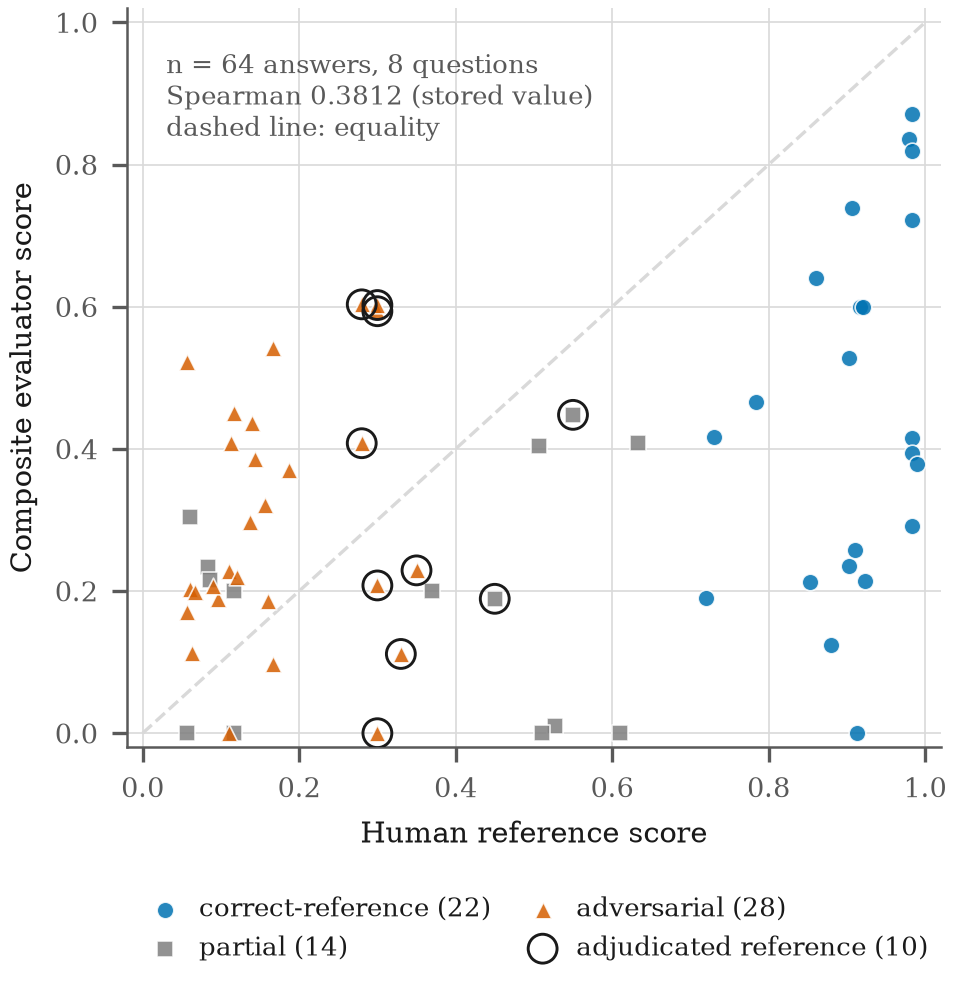
\includegraphics[width=0.85\linewidth]{IEEE_Figures/fig2_evaluator_scatter.png}
\caption{Composite evaluator score vs. human reference score, 64 constructed answers. The dashed line marks equality.}
\label{fig:scatter}
\end{figure}

The full composite correlates \emph{below} the cross-encoder alone, consistent with its safety-hardened design. A trivial word-count baseline matches the cross-encoder's correlation on this benchmark -- an unflattering result reported rather than omitted. We treat the human-correlation result as exploratory and initial evidence, not a validated accuracy claim.

\subsection{RL Baseline Comparison and Confirmatory Equivalence}
\label{sec:rlresults}

Table~\ref{tab:rl} reports tracking MAE; lower is better.

\begin{table}[t]
\caption{Difficulty-tracking error by condition (5 personas $\times$ 5 seeds)}
\label{tab:rl}
\centering
\begin{tabular}{lc}
\toprule
Condition & Tracking MAE \\
\midrule
Fixed difficulty & 1.200 \\
Rule-based heuristic & 0.473 \\
PPO (raw policy) & 0.804 \\
PPO + guardrails & 0.677 \\
\bottomrule
\end{tabular}
\end{table}

The rule-based heuristic outperforms every PPO variant. The pre-registered confirmatory test gives a 95\% CI for PPO-plus-guardrails minus constant-action-plus-guardrails that crosses zero (Fig.~\ref{fig:equiv}) -- the trained policy's contribution beyond the guardrail shield is not statistically distinguishable from zero, and the policy is measurably more volatile than the constant action under the same shield. We report this as a genuine, pre-registered equivalence finding.

\begin{figure}[t]
\centering
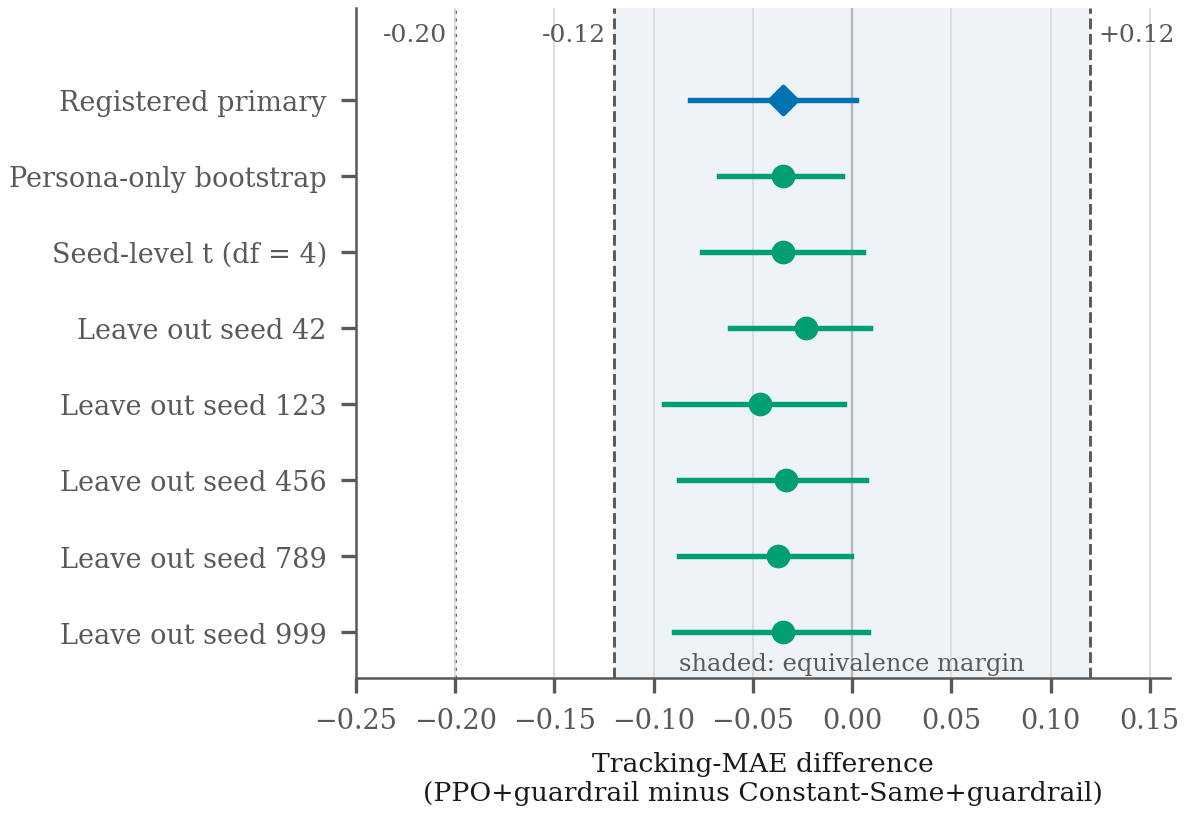
\includegraphics[width=0.85\linewidth]{IEEE_Figures/fig3_equivalence.png}
\caption{Tracking-MAE difference (PPO+guardrails minus constant-action+guardrails) across the primary estimator and six robustness checks. The shaded band is the pre-registered equivalence margin.}
\label{fig:equiv}
\end{figure}

\subsection{Guardrail Verification and Testing}

Boundary testing found performance scores in $[0.30, 0.40)$ unguarded against a policy-proposed escalation. A single-condition threshold widening closed the gap (13/13 boundary cases passing, zero regressions across 283 tests).

\subsection{System Testing Summary}

A broader testing programme exercised the API contract, database integrity, adversarial input handling, and sandbox configuration, alongside a second defect (a Unicode launcher crash, fixed and regression-verified). 264/283 tests pass (93.3\%); all 19 remaining failures trace to one unavailable external dependency or one pre-existing documented issue.

\begin{table}[t]
\caption{Supporting system verification}
\centering
\begin{tabular}{p{2.1cm}p{3.0cm}p{1.9cm}}
\toprule
Area & Method & Result \\
\midrule
API contract & Direct test-client calls & 7/7 pass \\
Adversarial input & 10 edge-case texts & 10/10, no crash \\
DB integrity & Live-store inspection & 0/52, 0/26 orphaned \\
Sandbox config & Code inspection & All flags present \\
Frontend & Automated UI suite & 28/28 pass \\
\bottomrule
\end{tabular}
\end{table}

A later verification pass re-ran the full suite before and after three narrow, regression-verified fixes, confirming an identical 264/19/15 split -- zero regressions -- and independently confirmed via hash recomputation that the deployed and \S\ref{sec:rlresults}-evaluated PPO checkpoints are distinct, non-interchangeable artifacts. It also ran Gymnasium's standard \texttt{check\_env()} interface check.

\begin{table}[t]
\caption{Post-deployment verification evidence}
\centering
\begin{tabular}{p{3.6cm}p{3.4cm}}
\toprule
Check & Result \\
\midrule
Full regression suite, pre/post-fix & 264/19/15, zero regressions \\
Gymnasium \texttt{check\_env()} & Passed, no warnings \\
Checkpoint hash identity & Confirmed distinct, non-interchangeable \\
Qwen narrative-text quality & 1 defect fixed; 1 limitation disclosed \\
\bottomrule
\end{tabular}
\end{table}

\subsection{Limitations}

The cross-encoder's fine-tuning data is not fully recoverable. The human-correlation study uses researcher-constructed answers at modest scale. All RL evidence is simulation-based. No human-subject usability evaluation has been conducted. A rubric applied to the feedback LLM's generated text (distinct from its verified non-scoring role, \S\ref{sec:qwenverif}) found occasional factual imprecision and one hallucinated output field -- an open limitation.

\section{Conclusion and Future Work}

We presented PrepAIred and reported its full evidence record with uniform rigor regardless of outcome. The evaluator shows exploratory, moderate human correlation and is safety-hardened rather than accuracy-optimal; the embedded LLM is verified, not merely claimed, to be confined to feedback generation; and a pre-registered confirmatory test finds the PPO policy's marginal contribution over its own guardrail shield statistically indistinguishable from zero, while guardrail testing independently closed a genuine safety gap. Future work includes a larger, naturally elicited confirmatory human-correlation study; recovering or bounding the cross-encoder's fine-tuning provenance; and a reward formulation trained directly against the tracking metric.

\begin{thebibliography}{15}
\bibitem{karjus2026} A. Karjus et al., ``Machine-Assisted Grading of Nationwide School-Leaving Essay Exams with LLMs and Statistical NLP,'' arXiv:2601.16314, 2026.
\bibitem{mendonca2025} P. C. Mendon\c{c}a, F. Quintal, and F. Mendon\c{c}a, ``Evaluating LLMs for Automated Scoring in Formative Assessments,'' Applied Sciences, vol. 15, no. 5, Art. no. 2787, 2025, doi: 10.3390/app15052787.
\bibitem{wang2025} Y. Wang et al., ``AutoSCORE: Enhancing Automated Scoring with Multi-Agent Large Language Models via Structured Component Recognition,'' arXiv:2509.21910, 2025.
\bibitem{zhu2025} K. Zhu, H. Du et al., ``MultiAgentBench: Evaluating the Collaboration and Competition of LLM Agents,'' in Proc. ACL, vol. 1, pp. 8580--8622, 2025.
\bibitem{argos2026} Microsoft Research, ``Argos: Multimodal Reinforcement Learning with Agentic Verifier for AI Agents,'' arXiv:2512.03438, 2025.
\bibitem{schulman2017} J. Schulman, F. Wolski, P. Dhariwal, A. Radford, and O. Klimov, ``Proximal Policy Optimization Algorithms,'' arXiv:1707.06347, 2017.
\bibitem{reimers2019} N. Reimers and I. Gurevych, ``Sentence-BERT: Sentence Embeddings using Siamese BERT-Networks,'' in Proc. EMNLP, 2019.
\bibitem{johnson2019} J. Johnson, M. Douze, and H. J\'egou, ``Billion-Scale Similarity Search with GPUs,'' IEEE Trans. Big Data, vol. 7, no. 3, pp. 535--547, 2019.
\bibitem{weiss1982} D. J. Weiss, ``Improving Measurement Quality and Efficiency with Adaptive Testing,'' Applied Psychological Measurement, vol. 6, no. 4, pp. 473--492, 1982.
\bibitem{anderson1995} J. R. Anderson, A. T. Corbett, K. R. Koedinger, and R. Pelletier, ``Cognitive Tutors: Lessons Learned,'' The Journal of the Learning Sciences, vol. 4, no. 2, pp. 167--207, 1995.
\bibitem{corbett1994} A. T. Corbett and J. R. Anderson, ``Knowledge Tracing: Modeling the Acquisition of Procedural Knowledge,'' User Modeling and User-Adapted Interaction, vol. 4, no. 4, pp. 253--278, 1994.
\bibitem{graves2017} A. Graves, M. G. Bellemare, J. Menick, R. Munos, and K. Kavukcuoglu, ``Automated Curriculum Learning for Neural Networks,'' in Proc. ICML, 2017.
\bibitem{portelas2020} R. Portelas, C. Colas, L. Weng, K. Hofmann, and P. Y. Oudeyer, ``Automatic Curriculum Learning for Deep RL: A Short Survey,'' in Proc. IJCAI, 2020.
\bibitem{naim2015} I. Naim, M. I. Tanveer, D. Gildea, and M. E. Hoque, ``Automated Prediction and Analysis of Job Interview Performance: The Role of What You Say and How You Say It,'' in Proc. 11th IEEE Int. Conf. Workshops Automatic Face and Gesture Recognition (FG), 2015, doi: 10.1109/FG.2015.7163127.
\bibitem{chen2017} L. Chen, G. Feng, C. W. Leong, B. Lehman, and M. Martin-Raugh, ``Automated Scoring of Interview Videos Using Doc2Vec Multimodal Feature Extraction Paradigm,'' in Proc. 18th ACM Int. Conf. Multimodal Interaction (ICMI '16), 2016, doi: 10.1145/2993148.2993203.
\end{thebibliography}

\end{document}
